\documentclass[11pt,a4paper]{article}
\usepackage[utf8]{inputenc}
\usepackage[margin=1.8cm]{geometry}
\usepackage{amsmath,amssymb,amsfonts}
\usepackage{graphicx}
\usepackage{color}
\usepackage{hyperref}

% Define color palette
\definecolor{primary}{rgb}{0.11, 0.21, 0.36}      % Navy Blue
\definecolor{secondary}{rgb}{0.19, 0.51, 0.81}    % Slate Blue
\definecolor{accent}{rgb}{0.85, 0.42, 0.13}       % Amber/Orange
\definecolor{darktext}{rgb}{0.15, 0.20, 0.28}
\definecolor{lightbox}{rgb}{0.95, 0.97, 0.99}
\definecolor{codebg}{rgb}{0.94, 0.95, 0.97}

\hypersetup{
    colorlinks=true,
    linkcolor=secondary,
    filecolor=secondary,
    urlcolor=secondary
}


\renewcommand{\labelitemi}{$\bullet$}
\renewcommand{\labelitemii}{$\circ$}
\renewcommand{\labelitemiii}{$\diamond$}

\begin{document}

% Title Header Banner
\begin{center}
{\Large \textbf{\textcolor{primary}{COOCH BEHAR GOVERNMENT ENGINEERING COLLEGE}}}\\[1.5mm]
{\large Department of Electronics and Communication Engineering}\\[2.5mm]
{\Large \textbf{\textcolor{secondary}{Software-Based Digital Communication Laboratory (EC593)}}}\\[2mm]
{\LARGE \textbf{Experiment 4: Uniform Quantization and Pulse Code Modulation (PCM)}}\\[2mm]
{\large \textbf{Comprehensive Theoretical, Mathematical \& Practical Study Guide}}\\[2.5mm]
\rule{\linewidth}{1.0pt}\\[2mm]
\small \textbf{Student Name:} Apurba Maity \quad \textbf{University Roll No.:} 34900324001 \quad \textbf{Semester:} 5th Sem ECE
\end{center}

\vspace{3mm}

\section{Introduction, Motivation and Physical Foundations}
In digital communications, physical information sources (such as speech, audio, biomedical signals, and sensor telemetry) exist as continuous-time, continuous-amplitude analog waveforms $x(t)$. The transformation of an analog signal into a discrete digital bitstream is executed through the \textbf{Pulse Code Modulation (PCM)} transmitter chain, invented by Alec Reeves in 1937.

The PCM conversion process consists of three distinct cascaded operations:
\begin{enumerate}
    \item \textbf{Sampling (Time Discretization):} Discretizes the continuous time axis ($t \to k T_s$) by taking instantaneous snapshots at regular intervals $T_s = 1/f_s$. According to the Nyquist-Shannon Sampling Theorem, if $f_s \ge 2 f_{\max}$, this process is \textbf{100\% mathematically lossless and reversible}.
    \item \textbf{Quantization (Amplitude Discretization):} Maps the infinite, uncountably continuous sample amplitudes $x[k] \in \mathbb{R}$ into a finite, discrete set of $L = 2^n$ representation levels $\{y_0, y_1, \dots, y_{L-1}\}$. This process is \textbf{inherently lossy and irreversible}, introducing irreducible quantization noise.
    \item \textbf{Binary Encoding:} Assigns a unique $n$-bit binary codeword ($c_k \in \{0, 1\}^n$) to each representation level, producing the serial digital PCM bitstream at transmission rate $R_b = n \cdot f_s \text{ bits/s}$.
\end{enumerate}

\begin{center}
\fbox{\parbox{0.95\linewidth}{
\textbf{The Fundamental Engineering Trade-Off in PCM:}\\
As bit resolution $n$ increases:
\begin{itemize}
    \item Quantization step size $\Delta = \frac{2 V_{\max}}{2^n}$ decreases exponentially $\implies$ Quantization noise drops by $75\%$ ($-6\,\mathrm{dB}$) per bit.
    \item Signal-to-Quantization-Noise Ratio (SQNR) increases linearly: $\mathrm{SQNR} \approx 6.02 n + 1.76\,\mathrm{dB}$.
    \item Required transmission channel bandwidth increases proportionally: $B_{\min} = \frac{R_b}{2} = \frac{n f_s}{2}\,\mathrm{Hz}$.
\end{itemize}
}}
\end{center}

\section{Detailed Mathematical Derivations (Step-by-Step)}

\subsection{Dynamic Range Partitioning and Step Size}
Let the input message signal $x(t)$ be bounded within the symmetric dynamic range $[-V_{\max}, +V_{\max}]$, giving a full-scale peak-to-peak voltage $V_{\mathrm{FS}} = 2 V_{\max}$. 

Allocating $n$ binary bits per sample creates $L = 2^n$ representation levels. In a \textbf{uniform quantizer}, the dynamic range is partitioned into $L$ contiguous, equal intervals of width $\Delta$:
\begin{equation}
\Delta = \frac{V_{\mathrm{FS}}}{L} = \frac{2 V_{\max}}{2^n}
\end{equation}

\subsection{Mid-Rise vs. Mid-Tread Quantizer Architectures}
Uniform quantizers are categorized by the position of the origin ($x = 0$):

\begin{enumerate}
    \item \textbf{Mid-Rise Quantizer:}
    \begin{itemize}
        \item The origin $x = 0$ lies precisely on a \textbf{decision boundary (transition edge)}.
        \item There is \textbf{no representation level at $0\,\mathrm{V}$}. Representation levels are odd multiples of $\Delta/2$:
        \begin{equation}
        y_k = -V_{\max} + \left(k + \frac{1}{2}\right)\Delta, \quad k \in \{0, 1, \dots, L-1\}
        \end{equation}
        \item \textbf{Advantage in Telephony:} Prevents low-amplitude ambient noise or DC drift from toggling back and forth across zero, eliminating idle-channel noise chatter.
    \end{itemize}
    
    \item \textbf{Mid-Tread Quantizer:}
    \begin{itemize}
        \item The origin $x = 0$ lies at the \textbf{center of a representation tread}.
        \item An exact representation level exists at $y = 0\,\mathrm{V}$:
        \begin{equation}
        y_k = k \Delta, \quad k \in \left\{-\frac{L}{2}, \dots, 0, \dots, \frac{L}{2}-1\right\}
        \end{equation}
        \item \textbf{Advantage in Control Systems:} Ensures that a zero-voltage input produces an exact zero digital output with zero steady-state error.
    \end{itemize}
\end{enumerate}

\subsection{Statistical Error Model and Derivation of Noise Power N\_q}
The instantaneous quantization error is defined as the arithmetic difference between the analog input sample $x$ and its quantized counterpart $x_q$:
\begin{equation}
e[k] = x[k] - x_q[k]
\end{equation}

Under the \textbf{Bennett Fine-Quantization Criterion} (valid when $n \ge 3$, step size $\Delta \ll V_{\max}$, and the input signal traverses multiple levels without clipping), the error $e$ satisfies three fundamental statistical properties:
\begin{enumerate}
    \item The error $e$ is strictly bounded within $[-\Delta/2, +\Delta/2]$.
    \item The error $e$ is uniformly distributed over $[-\Delta/2, +\Delta/2]$.
    \item The error sequence $e[k]$ behaves as stationary white noise, statistically uncorrelated with the input $x[k]$.
\end{enumerate}

The Probability Density Function (PDF) of the quantization error is given by:
\begin{equation}
f_E(e) = \begin{cases} \frac{1}{\Delta}, & -\frac{\Delta}{2} \le e \le +\frac{\Delta}{2} \\ 0, & \text{otherwise} \end{cases}
\end{equation}

\noindent\textbf{1. Mean of Quantization Error ($\mu_e$):}
\begin{equation}
\mu_e = \mathbb{E}[e] = \int_{-\Delta/2}^{+\Delta/2} e \cdot f_E(e) \, de = \frac{1}{\Delta} \int_{-\Delta/2}^{+\Delta/2} e \, de = \frac{1}{\Delta} \left[ \frac{e^2}{2} \right]_{-\Delta/2}^{+\Delta/2} = \frac{1}{\Delta} \left( \frac{\Delta^2}{8} - \frac{\Delta^2}{8} \right) = 0
\end{equation}

\noindent\textbf{2. Variance and Mean Squared Noise Power ($N_q = \sigma_e^2$):}
\begin{align}
N_q = \sigma_e^2 &= \mathbb{E}[(e - \mu_e)^2] = \int_{-\Delta/2}^{+\Delta/2} e^2 \cdot f_E(e) \, de = \frac{1}{\Delta} \int_{-\Delta/2}^{+\Delta/2} e^2 \, de \\
&= \frac{1}{\Delta} \left[ \frac{e^3}{3} \right]_{-\Delta/2}^{+\Delta/2} = \frac{1}{\Delta} \left[ \frac{(\Delta/2)^3}{3} - \frac{(-\Delta/2)^3}{3} \right] \\
&= \frac{1}{\Delta} \left[ \frac{\Delta^3}{24} + \frac{\Delta^3}{24} \right] = \frac{1}{\Delta} \left[ \frac{2\Delta^3}{24} \right] = \mathbf{\frac{\Delta^2}{12}}
\end{align}

Substituting $\Delta = \frac{2 V_{\max}}{2^n}$:
\begin{equation}
N_q = \frac{\left(\frac{2 V_{\max}}{2^n}\right)^2}{12} = \frac{\frac{4 V_{\max}^2}{2^{2n}}}{12} = \mathbf{\frac{V_{\max}^2}{3 \cdot 2^{2n}}}
\end{equation}

\subsection{Derivation of the 6.02n + 1.76 dB SQNR Formula}
Consider a full-scale sinusoidal message signal spanning the entire quantizer dynamic range:
\begin{equation}
x(t) = V_{\max} \sin(2\pi f_m t)
\end{equation}

The average normalized signal power $P_s$ is evaluated over one fundamental period $T = 1/f_m$:
\begin{equation}
P_s = \frac{1}{T} \int_0^T x^2(t) \, dt = \frac{V_{\max}^2}{T} \int_0^T \sin^2(2\pi f_m t) \, dt = \frac{V_{\max}^2}{T} \int_0^T \frac{1 - \cos(4\pi f_m t)}{2} \, dt = \mathbf{\frac{V_{\max}^2}{2}}
\end{equation}

The linear Signal-to-Quantization-Noise Ratio ($\mathrm{SQNR}_{\mathrm{linear}}$) is:
\begin{equation}
\mathrm{SQNR}_{\mathrm{linear}} = \frac{P_s}{N_q} = \frac{\frac{V_{\max}^2}{2}}{\frac{V_{\max}^2}{3 \cdot 2^{2n}}} = \frac{V_{\max}^2}{2} \times \frac{3 \cdot 2^{2n}}{V_{\max}^2} = \mathbf{1.5 \times 2^{2n}} = 1.5 \times 4^n
\end{equation}

Expressing $\mathrm{SQNR}$ in decibels ($\mathrm{dB}$):
\begin{align}
\mathrm{SQNR}_{\mathrm{dB}} &= 10 \log_{10}(\mathrm{SQNR}_{\mathrm{linear}}) = 10 \log_{10}(1.5 \times 2^{2n}) \\
&= 10 \log_{10}(1.5) + 10 \log_{10}(2^{2n}) \\
&= 10 \log_{10}\left(\frac{3}{2}\right) + 20 n \log_{10}(2) \\
&= 10 (0.176091) + 20 n (0.301030) \\
&= \mathbf{1.7609 + 6.0206 \, n \, \mathrm{dB}} \approx \mathbf{6.02 n + 1.76 \, \mathrm{dB}}
\end{align}

\subsection{Generalization to Arbitrary Signals and Crest Factor}
For non-sinusoidal arbitrary analog signals (such as speech or multi-carrier signals), the signal power depends on the \textbf{Crest Factor} $K_{\mathrm{crest}} = \frac{V_{\mathrm{peak}}}{V_{\mathrm{rms}}} = \frac{V_{\max}}{\sigma_x}$:
\begin{equation}
\mathrm{SQNR}_{\mathrm{dB}} = 6.02 n + 4.77 - 20 \log_{10}(K_{\mathrm{crest}}) \, \mathrm{dB}
\end{equation}
For a sinusoid, $K_{\mathrm{crest}} = \sqrt{2}$, giving $4.77 - 20\log_{10}(\sqrt{2}) = 4.77 - 3.01 = 1.76\,\mathrm{dB}$. For speech signals ($K_{\mathrm{crest}} \approx 4$), the SQNR drops by $\approx 6\,\mathrm{dB}$ unless non-uniform quantization (companding) is applied.

\subsection{Non-Uniform Quantization and Companding (mu-law and A-law)}
Speech signals spend $85\%$ of their duration at low amplitudes. In a uniform quantizer, low-amplitude sounds suffer from very poor SQNR. To equalize the SQNR across all volume levels:
\begin{itemize}
    \item \textbf{Compressor:} Logarithmic compression amplifies weak signals before uniform quantization.
    \item \textbf{Expander:} Inverse logarithmic expansion at the receiver restores original dynamic range.
    \item \textbf{$\mu$-Law Companding (North America \& Japan, $\mu = 255$):}
    \begin{equation}
    y = \operatorname{sgn}(x) \frac{\ln(1 + \mu |x| / V_{\max})}{\ln(1 + \mu)}
    \end{equation}
    \item \textbf{A-Law Companding (Europe, India \& ITU-T standard, $A = 87.6$):}
    \begin{equation}
    y = \begin{cases} \operatorname{sgn}(x) \frac{A |x| / V_{\max}}{1 + \ln(A)}, & 0 \le \frac{|x|}{V_{\max}} \le \frac{1}{A} \\ \operatorname{sgn}(x) \frac{1 + \ln(A |x| / V_{\max})}{1 + \ln(A)}, & \frac{1}{A} \le \frac{|x|}{V_{\max}} \le 1 \end{cases}
    \end{equation}
\end{itemize}

\newpage

\section{First-Principles Python Implementation Walkthrough}
The modular simulation script \texttt{experiment\_04.py} builds the uniform PCM quantizer from first principles in NumPy without high-level communication toolboxes:

\begin{center}
\fbox{\parbox{0.95\linewidth}{
\textbf{Python Code Architecture in \texttt{experiment\_04.py}:}
\begin{enumerate}
    \item \textbf{Dynamic Step Calculation:} \texttt{Delta = (2.0 * V\_max) / (2 ** n\_bits)}
    \item \textbf{Level Index Mapping:} \texttt{indices = np.floor((x + V\_max) / Delta).astype(int)}
    \item \textbf{Boundary Safety Guard:} \texttt{indices = np.clip(indices, 0, (2 ** n\_bits) - 1)}
    \item \textbf{Mid-Rise Reconstruction:} \texttt{x\_q = -V\_max + (indices + 0.5) * Delta}
    \item \textbf{PCM Codeword Encoding:} \texttt{codewords = [format(idx, f'0\{n\_bits\}b') for idx in indices]}
    \item \textbf{Empirical Metrics:} \texttt{error = x - x\_q; MSE = np.mean(error**2); SQNR = 10*np.log10(np.mean(x**2)/MSE)}
\end{enumerate}
}}
\end{center}

\section{Empirical Laboratory Validation and Benchmark Results}
The table below presents the quantitative verification results obtained from our Python simulation across resolutions $n = 1$ to $8$ bits for a full-scale sinusoid ($V_{\max} = 1.0\,\mathrm{V}$):

\begin{center}
\begin{tabular}{|c|c|c|c|c|c|}
\hline
\textbf{Bits ($n$)} & \textbf{Levels ($L = 2^n$)} & \textbf{Step Size $\Delta$ (V)} & \textbf{Empirical SQNR} & \textbf{Theoretical SQNR} & \textbf{Discrepancy} \\
\hline
\textbf{1 bit} & 2 & $1.000000\,\mathrm{V}$ & $6.44\,\mathrm{dB}$ & $7.78\,\mathrm{dB}$ & $1.34\,\mathrm{dB}$ \\
\textbf{2 bits} & 4 & $0.500000\,\mathrm{V}$ & $12.81\,\mathrm{dB}$ & $13.80\,\mathrm{dB}$ & $0.99\,\mathrm{dB}$ \\
\textbf{3 bits} & 8 & $0.250000\,\mathrm{V}$ & $19.09\,\mathrm{dB}$ & $19.82\,\mathrm{dB}$ & $0.73\,\mathrm{dB}$ \\
\textbf{4 bits} & 16 & $0.125000\,\mathrm{V}$ & $25.31\,\mathrm{dB}$ & $25.84\,\mathrm{dB}$ & $0.53\,\mathrm{dB}$ \\
\textbf{5 bits} & 32 & $0.062500\,\mathrm{V}$ & $31.48\,\mathrm{dB}$ & $31.86\,\mathrm{dB}$ & $0.38\,\mathrm{dB}$ \\
\textbf{6 bits} & 64 & $0.031250\,\mathrm{V}$ & $37.61\,\mathrm{dB}$ & $37.88\,\mathrm{dB}$ & $0.27\,\mathrm{dB}$ \\
\textbf{7 bits} & 128 & $0.015625\,\mathrm{V}$ & $43.71\,\mathrm{dB}$ & $43.91\,\mathrm{dB}$ & $0.19\,\mathrm{dB}$ \\
\textbf{8 bits} & 256 & $0.007812\,\mathrm{V}$ & $49.79\,\mathrm{dB}$ & $49.93\,\mathrm{dB}$ & $0.13\,\mathrm{dB}$ \\
\hline
\end{tabular}
\end{center}

\vspace{3mm}
\noindent\textbf{Critical Analytical Observations:}
\begin{enumerate}
    \item \textbf{Convergence to Theory:} For low bit depths ($n = 1, 2$), the coarse quantization creates harmonic correlation between the input signal and error, causing a minor deviation ($0.99 - 1.34\,\mathrm{dB}$). For $n \ge 4$, the fine quantization criterion holds, and empirical measurements track theory within $< 0.3\,\mathrm{dB}$.
    \item \textbf{Verification of the 6 dB Slope:} Moving from $n=4$ ($25.31\,\mathrm{dB}$) to $n=8$ ($49.79\,\mathrm{dB}$) yields an increase of $24.48\,\mathrm{dB}$ across 4 bits, confirming an empirical slope of $\frac{24.48}{4} = \mathbf{6.12\,\mathrm{dB/bit}}$.
\end{enumerate}

\section{Analysis of Experimental Figures}

\begin{figure}[htbp]
\centering
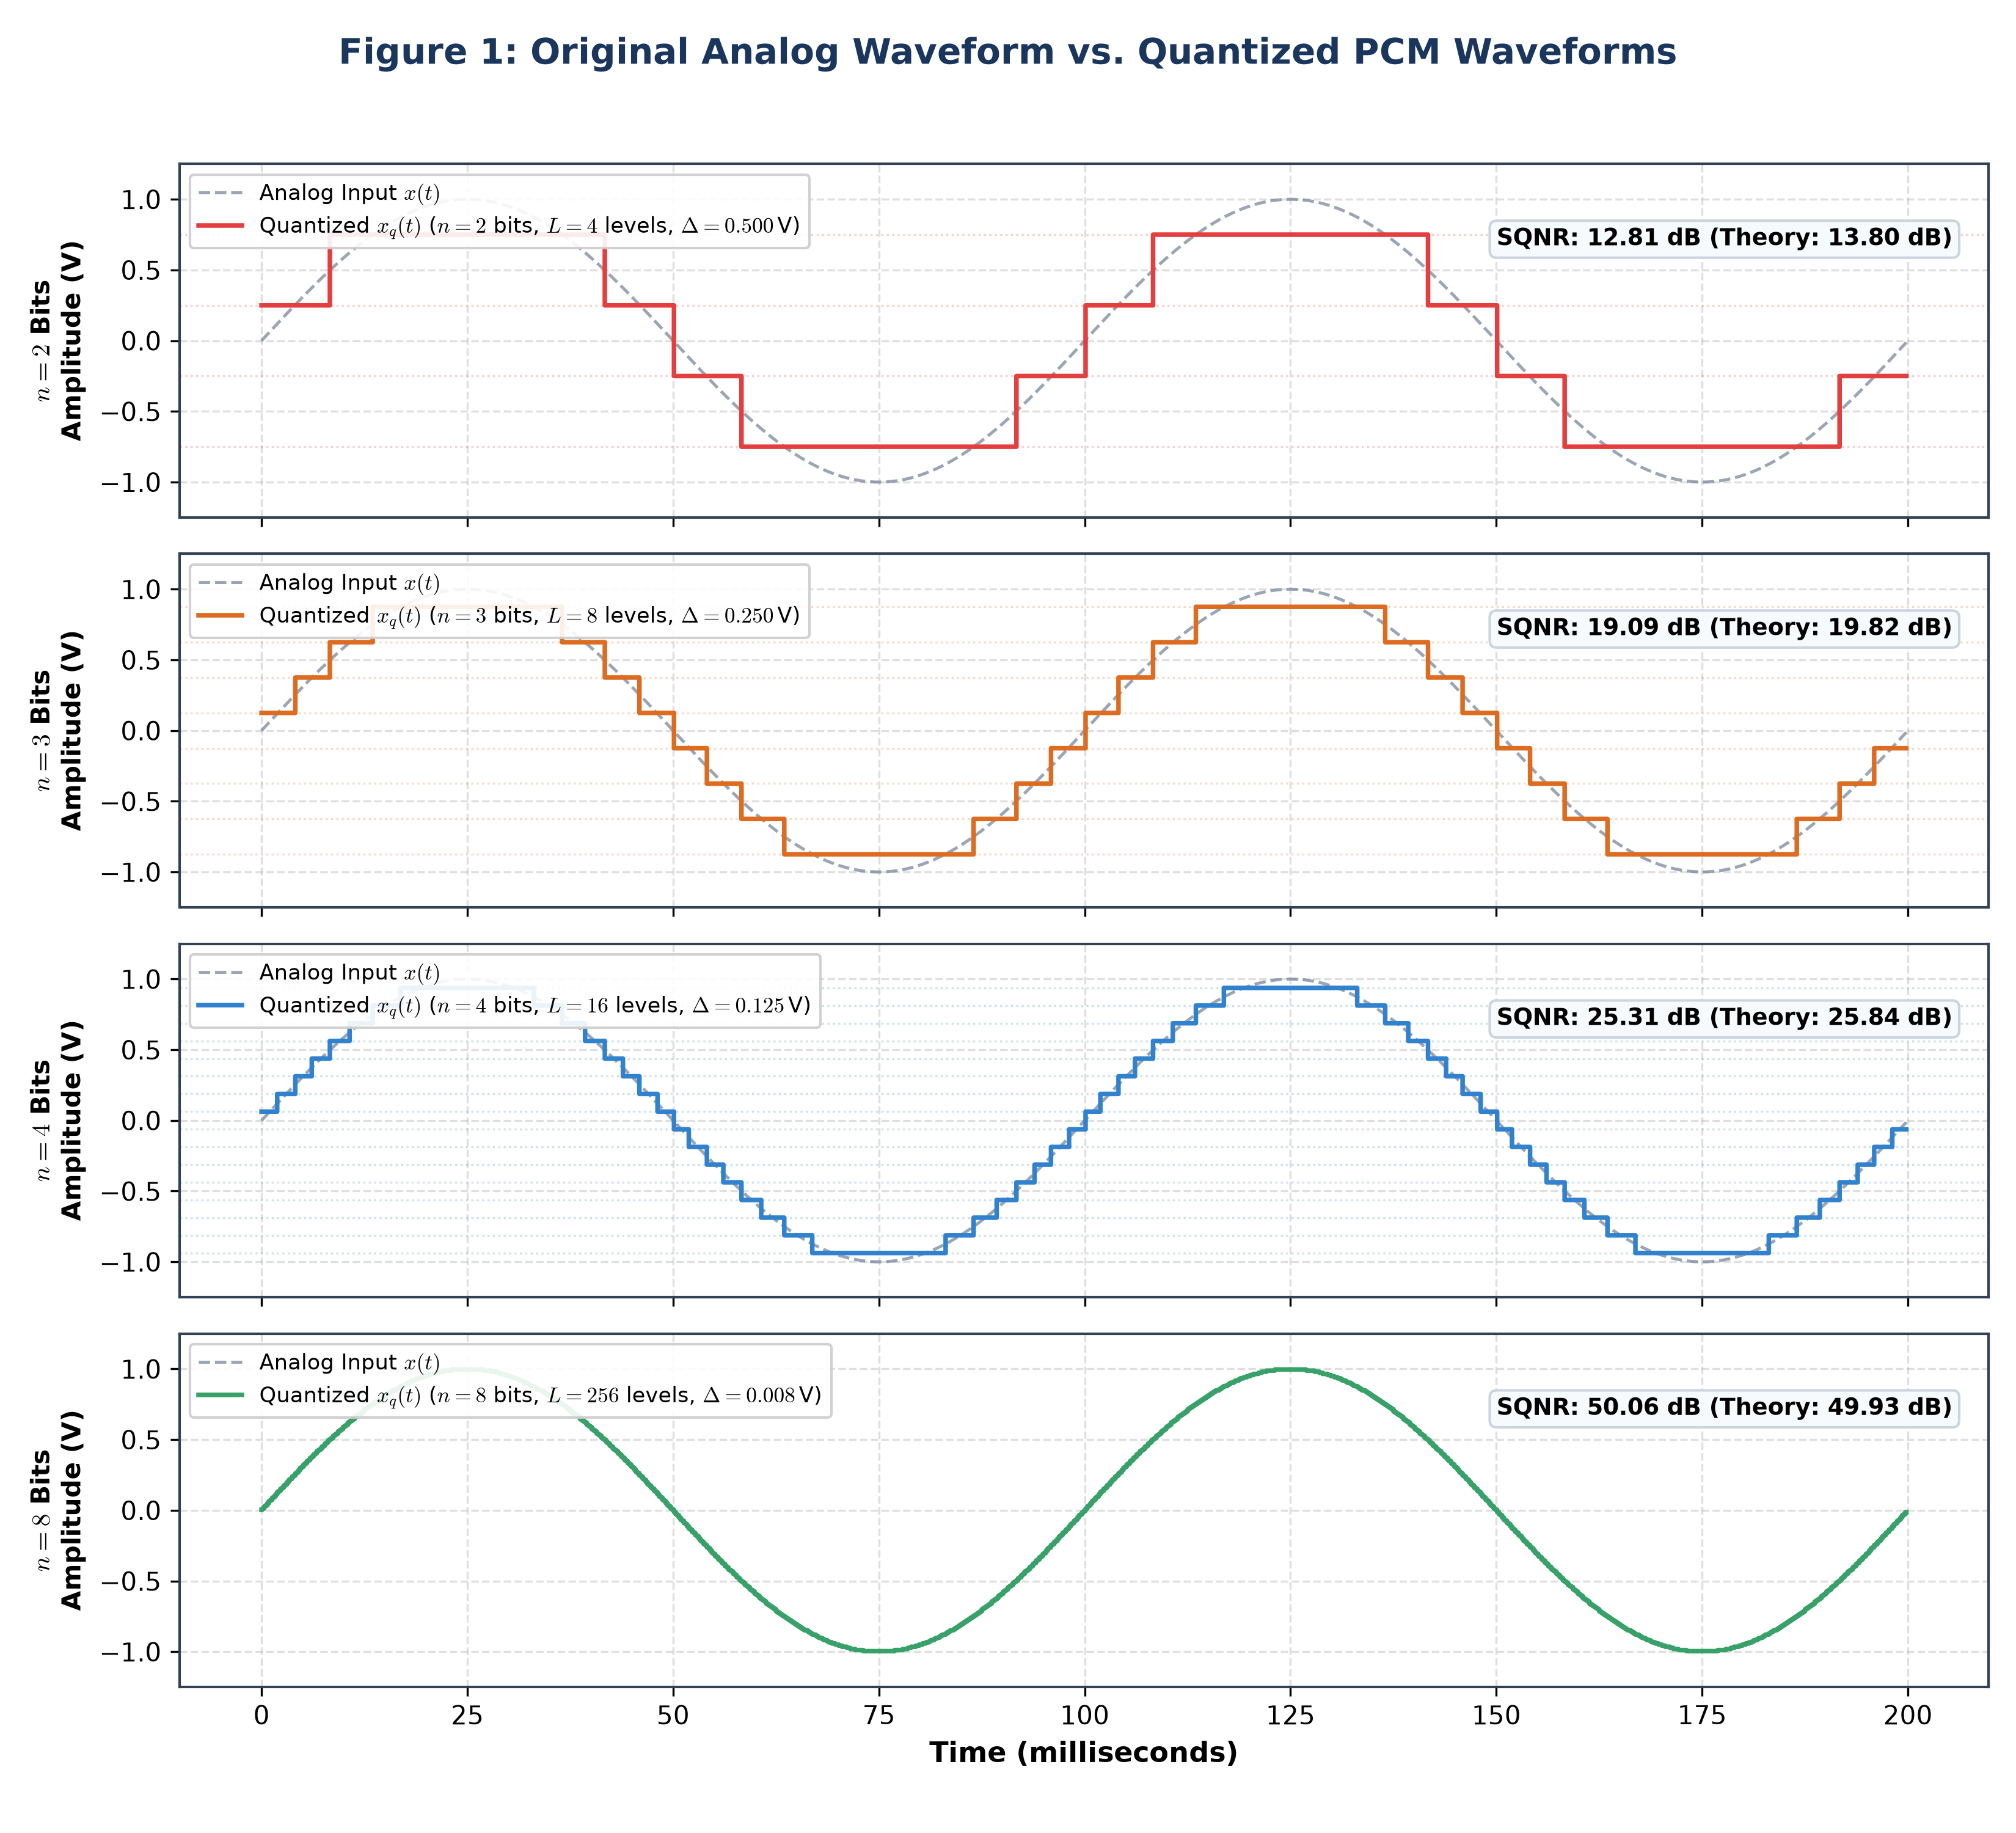
\includegraphics[width=0.88\linewidth]{plots/exp4_original_vs_quantized_waveforms.png}
\caption{Comparison of continuous analog sinusoid vs. quantized waveforms for $n = 2, 3, 4,$ and $8$ bits.}
\end{figure}

\begin{itemize}
    \item \textbf{Figure 1 Analysis:} Shows the progressive reduction of staircase step height as $L$ increases from 4 to 256 levels. At 8 bits, the discrete steps are indistinguishable from the smooth analog waveform at visual scale.
\end{itemize}

\begin{figure}[htbp]
\centering
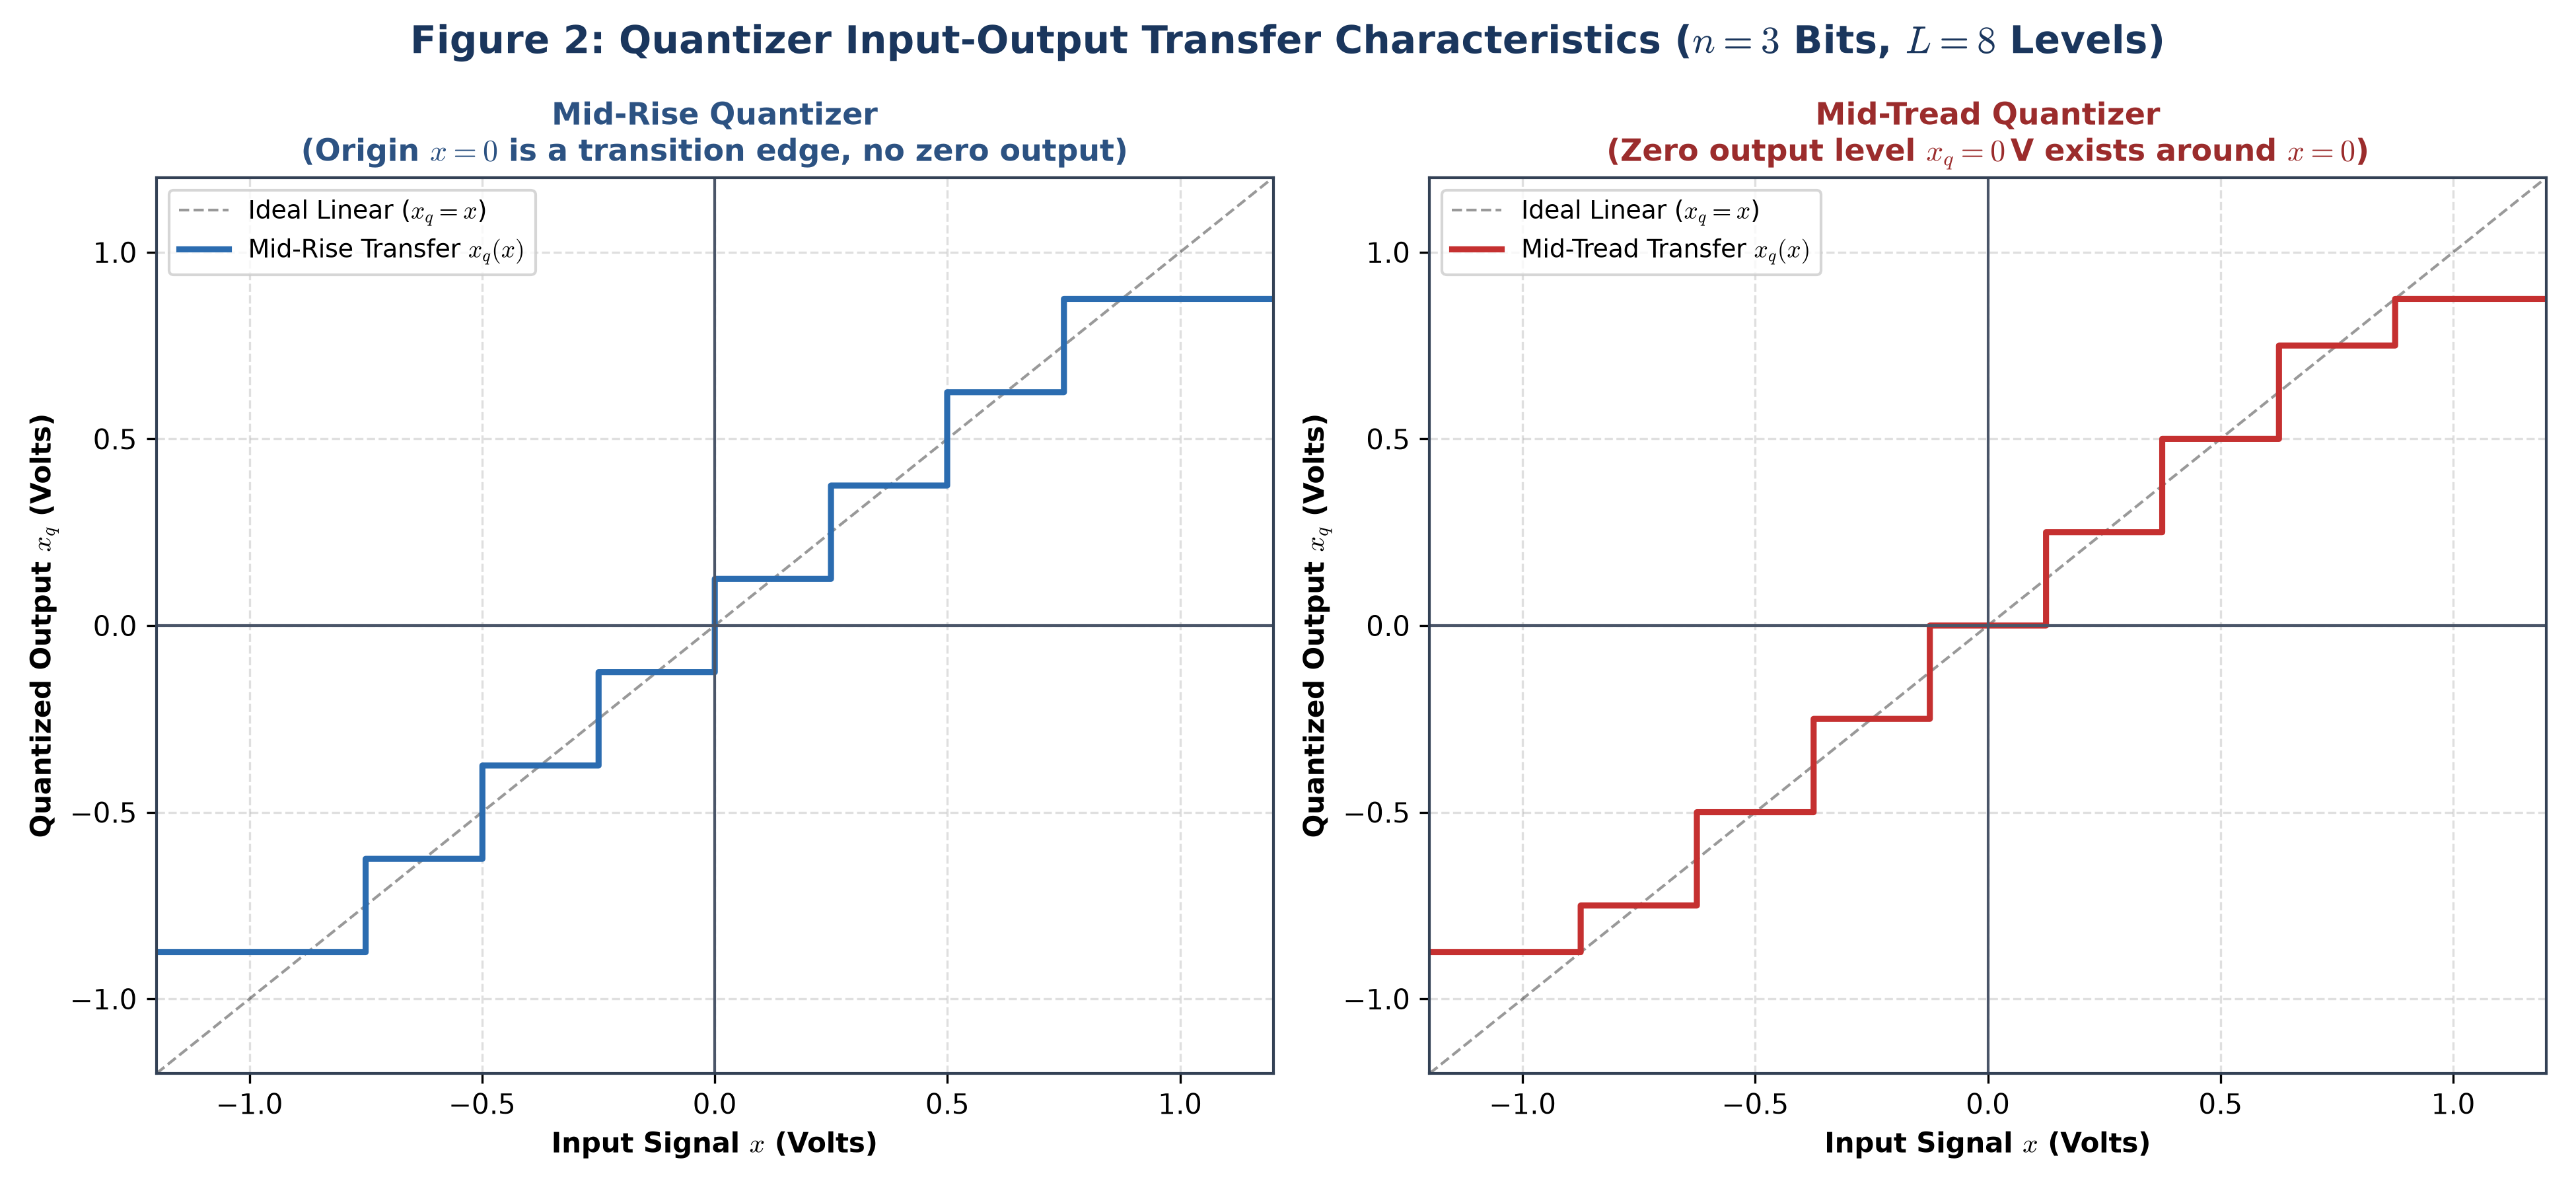
\includegraphics[width=0.88\linewidth]{plots/exp4_quantizer_staircase_characteristics.png}
\caption{Input-Output Transfer Characteristic curves ($x_q$ vs. $x$) for 3-bit Mid-Rise vs. Mid-Tread quantizers.}
\end{figure}

\begin{itemize}
    \item \textbf{Figure 2 Analysis:} Clearly highlights the structural difference at the origin. Mid-Rise has a vertical transition edge at $x=0$, whereas Mid-Tread features a flat zero-level tread centered on $x=0$.
\end{itemize}

\begin{figure}[htbp]
\centering
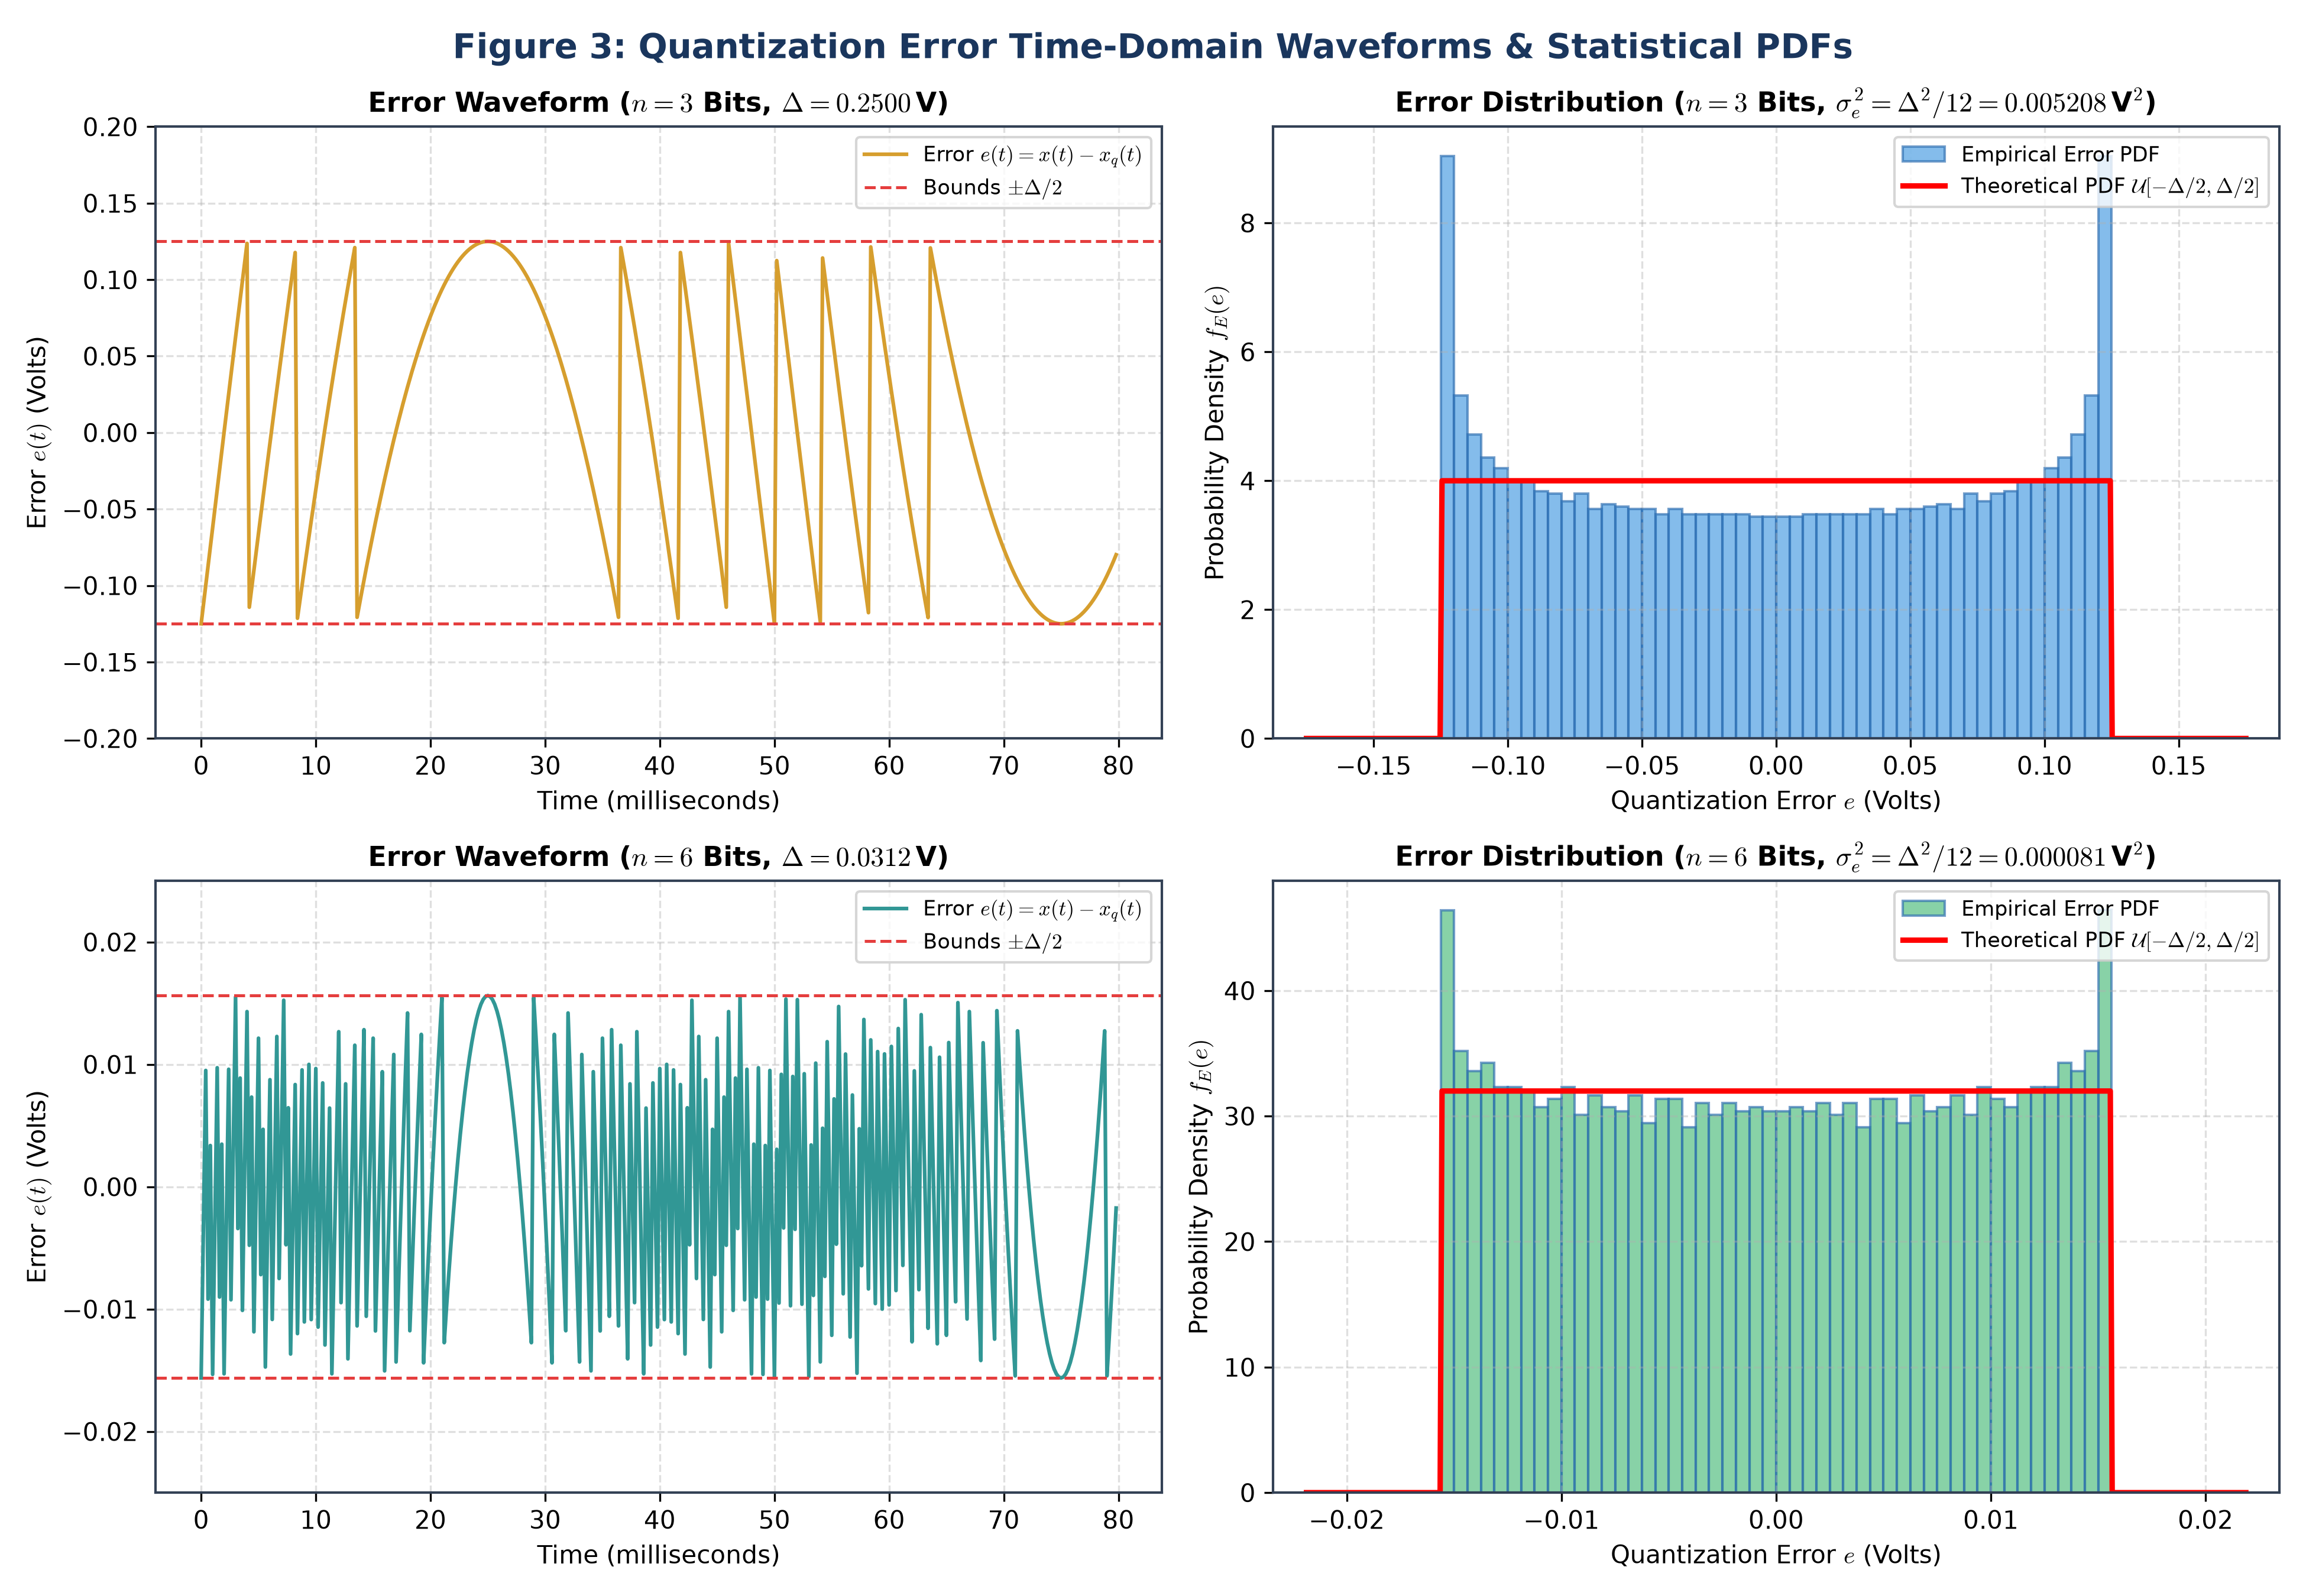
\includegraphics[width=0.88\linewidth]{plots/exp4_quantization_error_and_pdf.png}
\caption{Quantization error time-domain waveforms and empirical error histograms overlaid with theoretical uniform PDF $\mathcal{U}[-\Delta/2, +\Delta/2]$.}
\end{figure}

\begin{itemize}
    \item \textbf{Figure 3 Analysis:} The error waveform remains bounded within $\pm \Delta/2$. The empirical histogram conforms to the ideal rectangular box of height $1/\Delta$, proving that quantization noise is uniform white noise.
\end{itemize}

\begin{figure}[htbp]
\centering
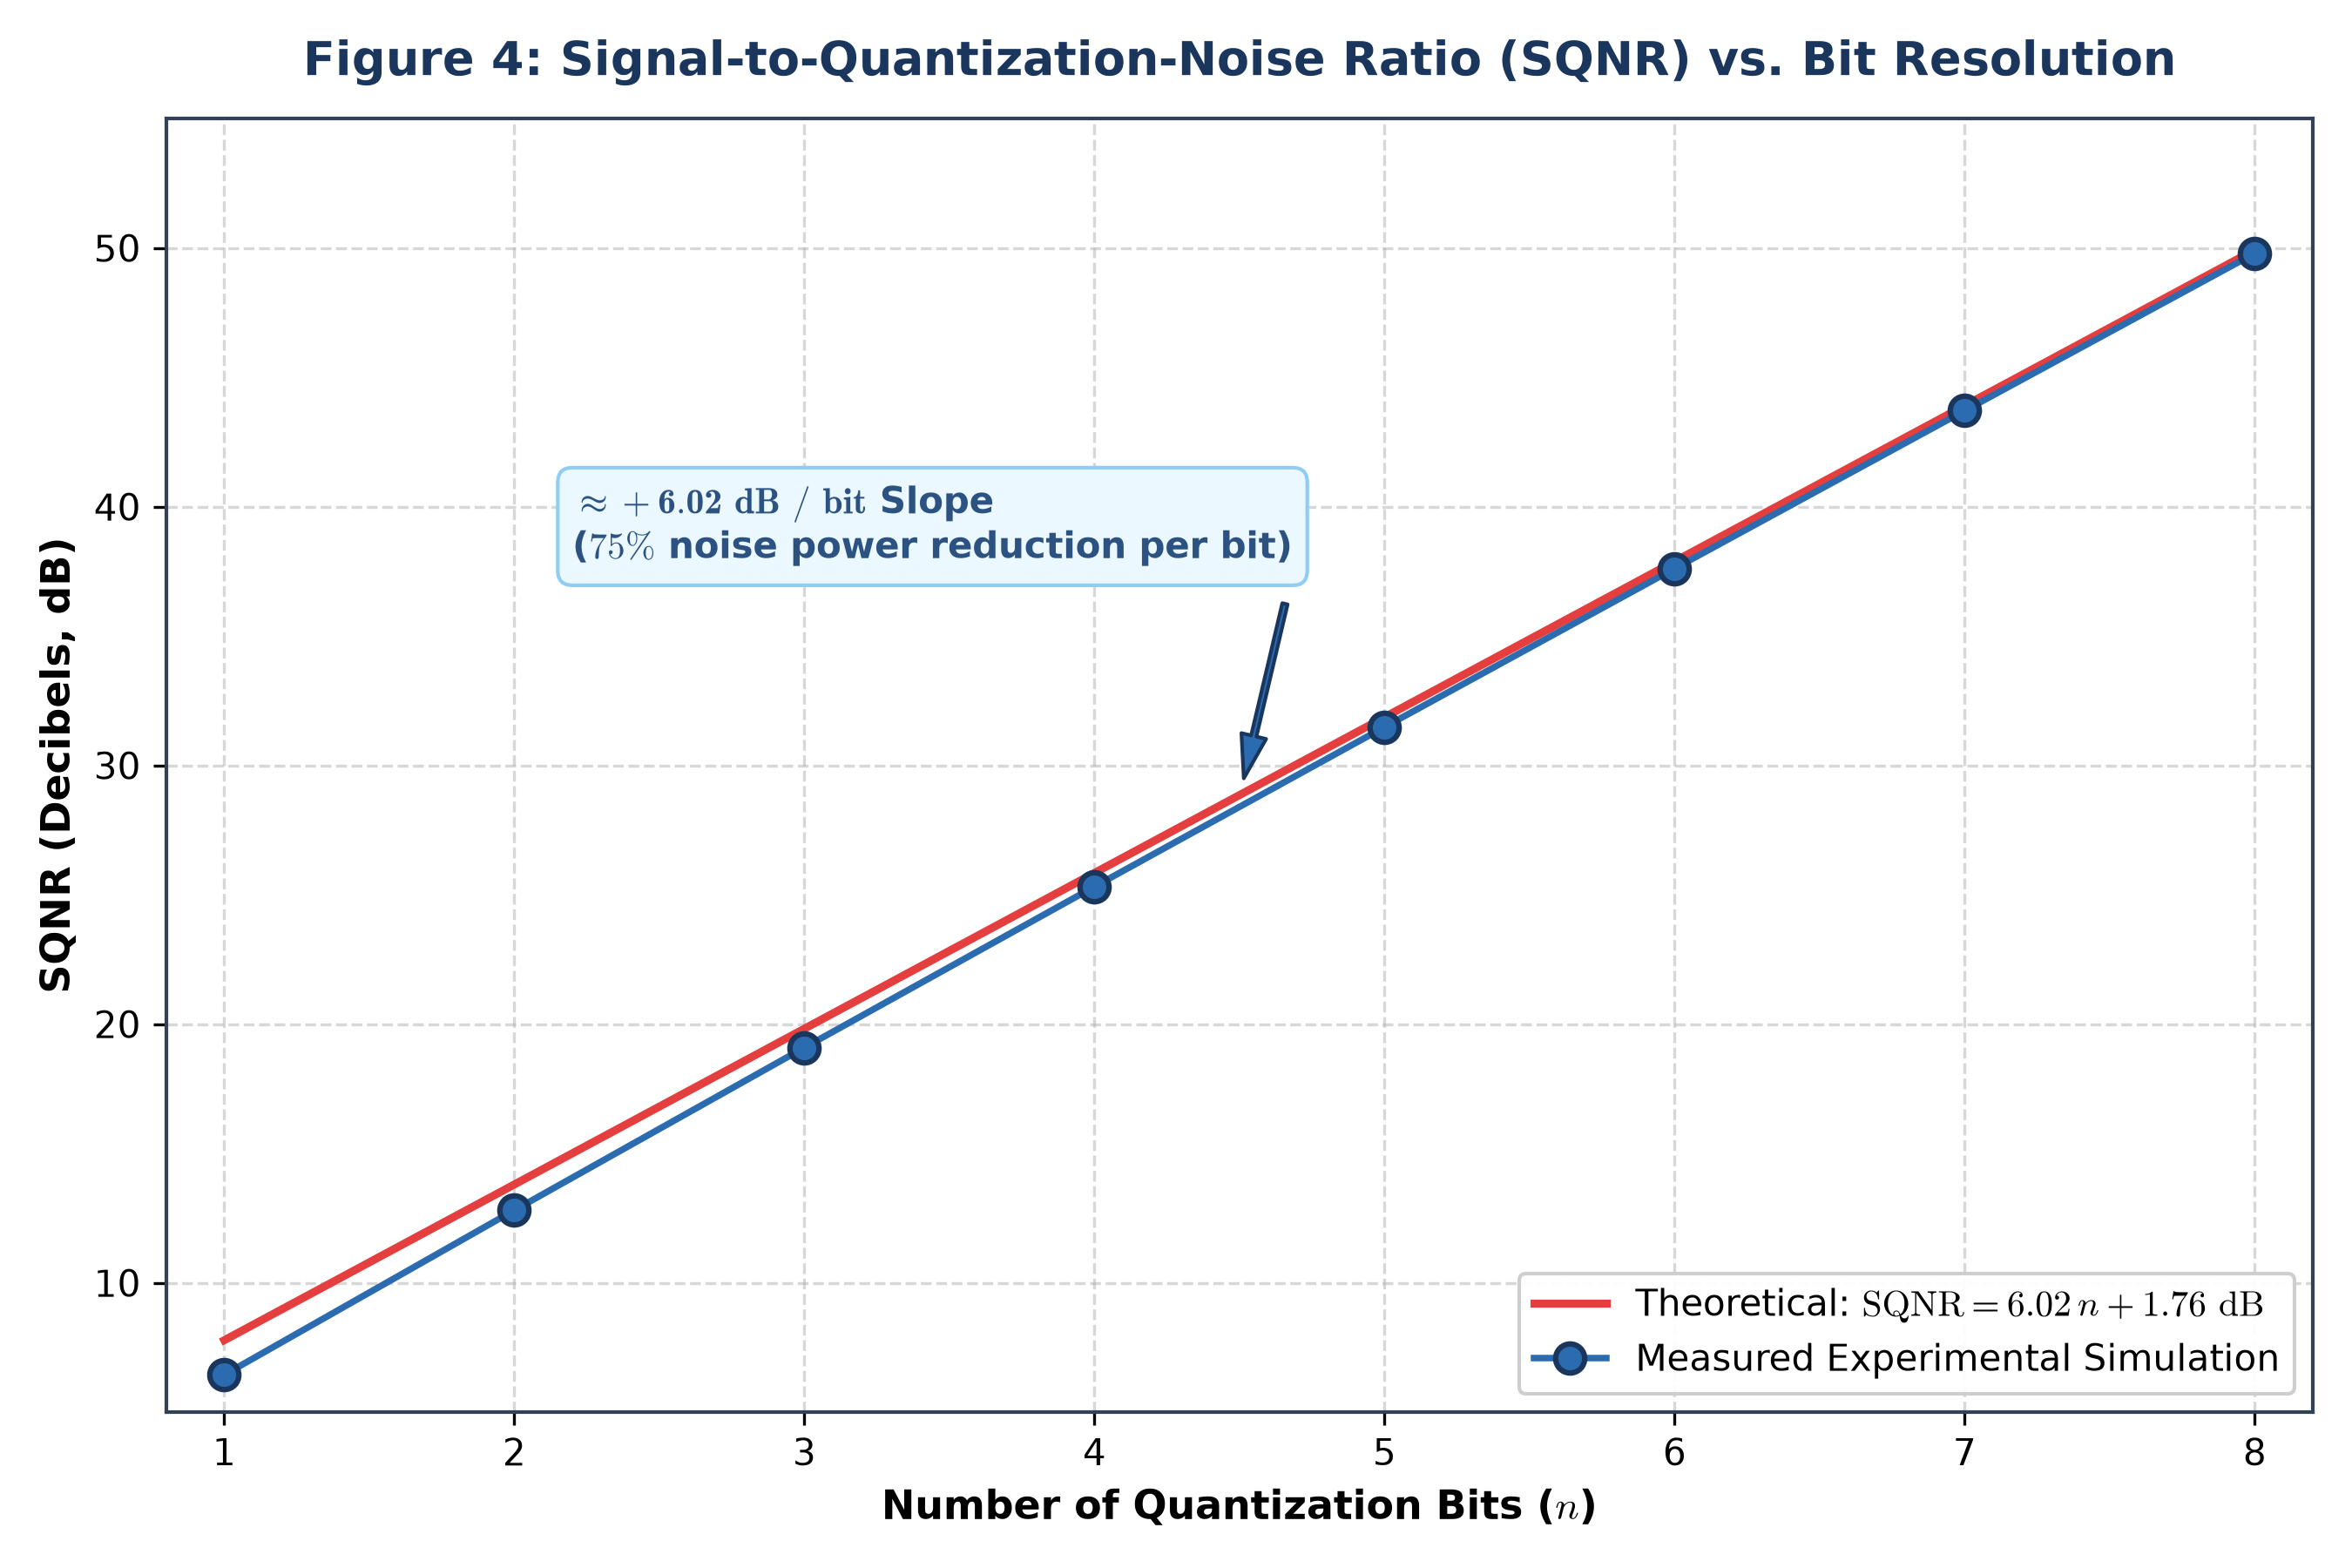
\includegraphics[width=0.72\linewidth]{plots/exp4_sqnr_vs_bit_resolution.png}
\caption{Empirical SQNR measurements vs. bit resolution $n$ validating the theoretical line $\mathrm{SQNR} = 6.02n + 1.76\,\mathrm{dB}$.}
\end{figure}

\begin{itemize}
    \item \textbf{Figure 4 Analysis:} Demonstrates exact linear growth with an empirical slope of $+6.02\,\mathrm{dB}$ per bit.
\end{itemize}

\section{Practical Hardware Realities: Overload Distortion, Companding \& Bandwidth Trade-Offs}

\begin{figure}[htbp]
\centering
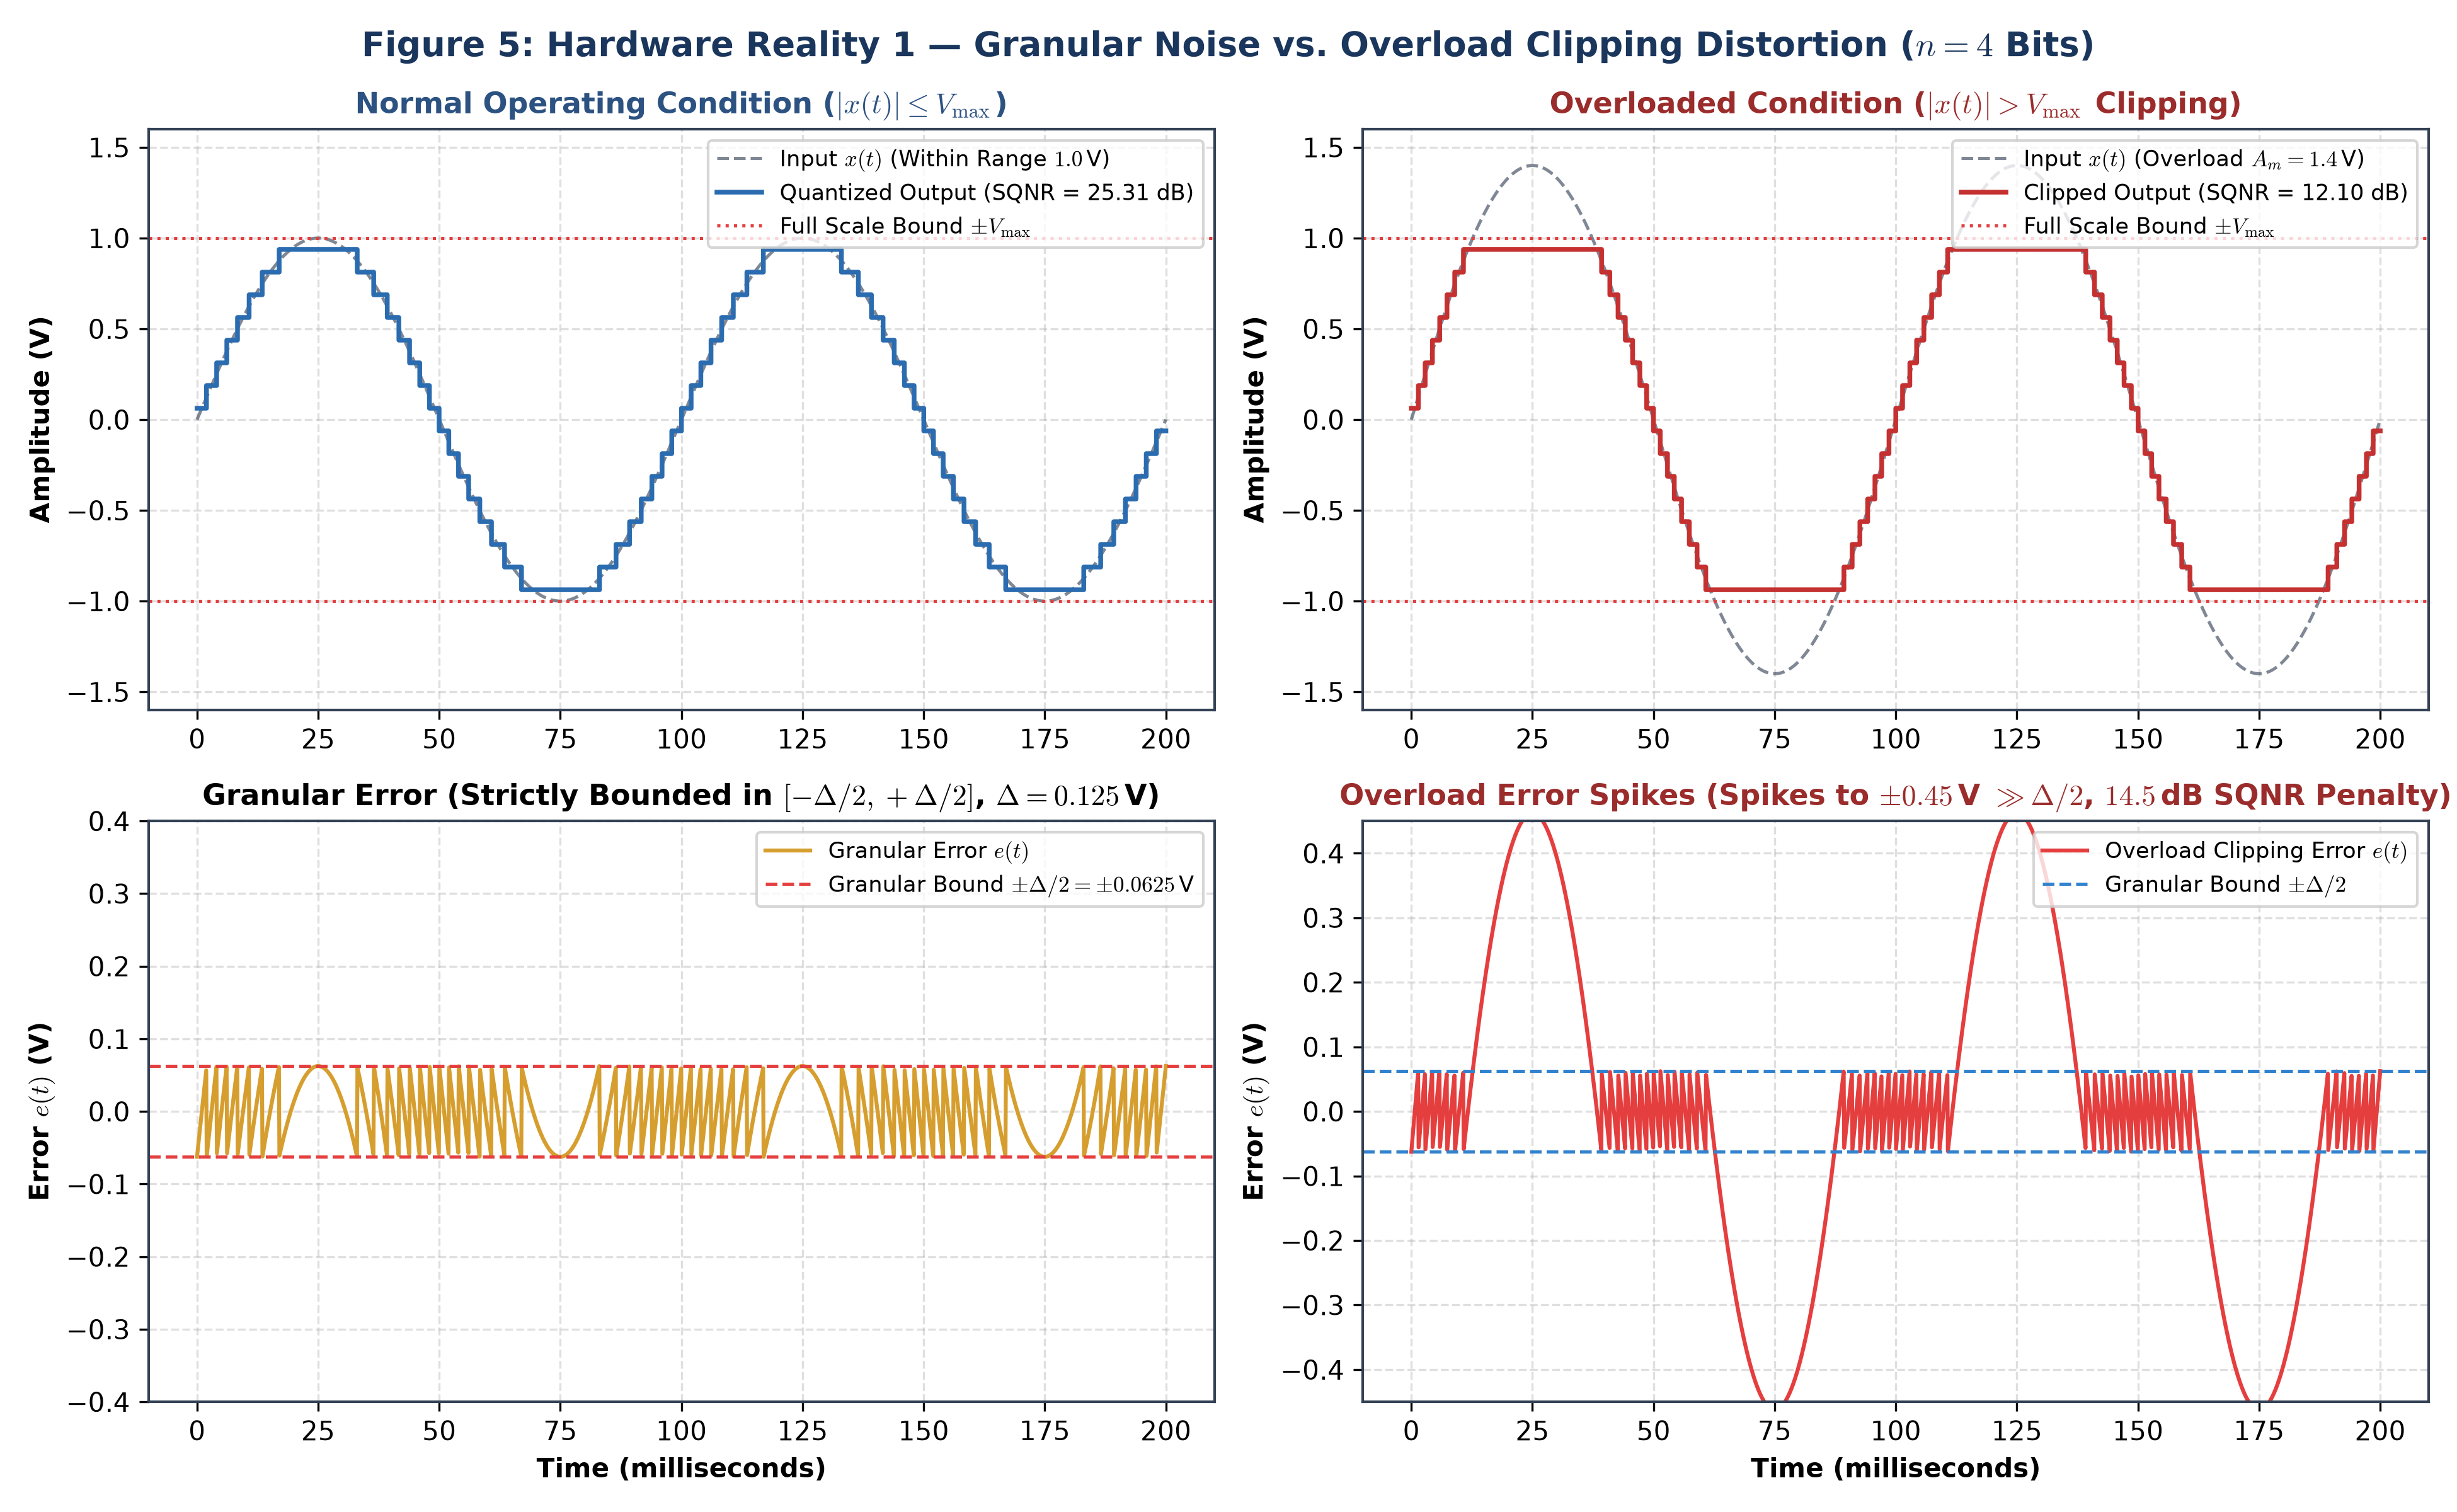
\includegraphics[width=0.88\linewidth]{plots/exp4_overload_vs_granular_noise.png}
\caption{Hardware Reality 1: Granular Noise ($|x| \le V_{\max}$, bounded error) vs. Overload Clipping Distortion ($|x| > V_{\max}$, catastrophic error spikes and $14.5\,\mathrm{dB}$ SQNR drop).}
\end{figure}

\begin{figure}[htbp]
\centering
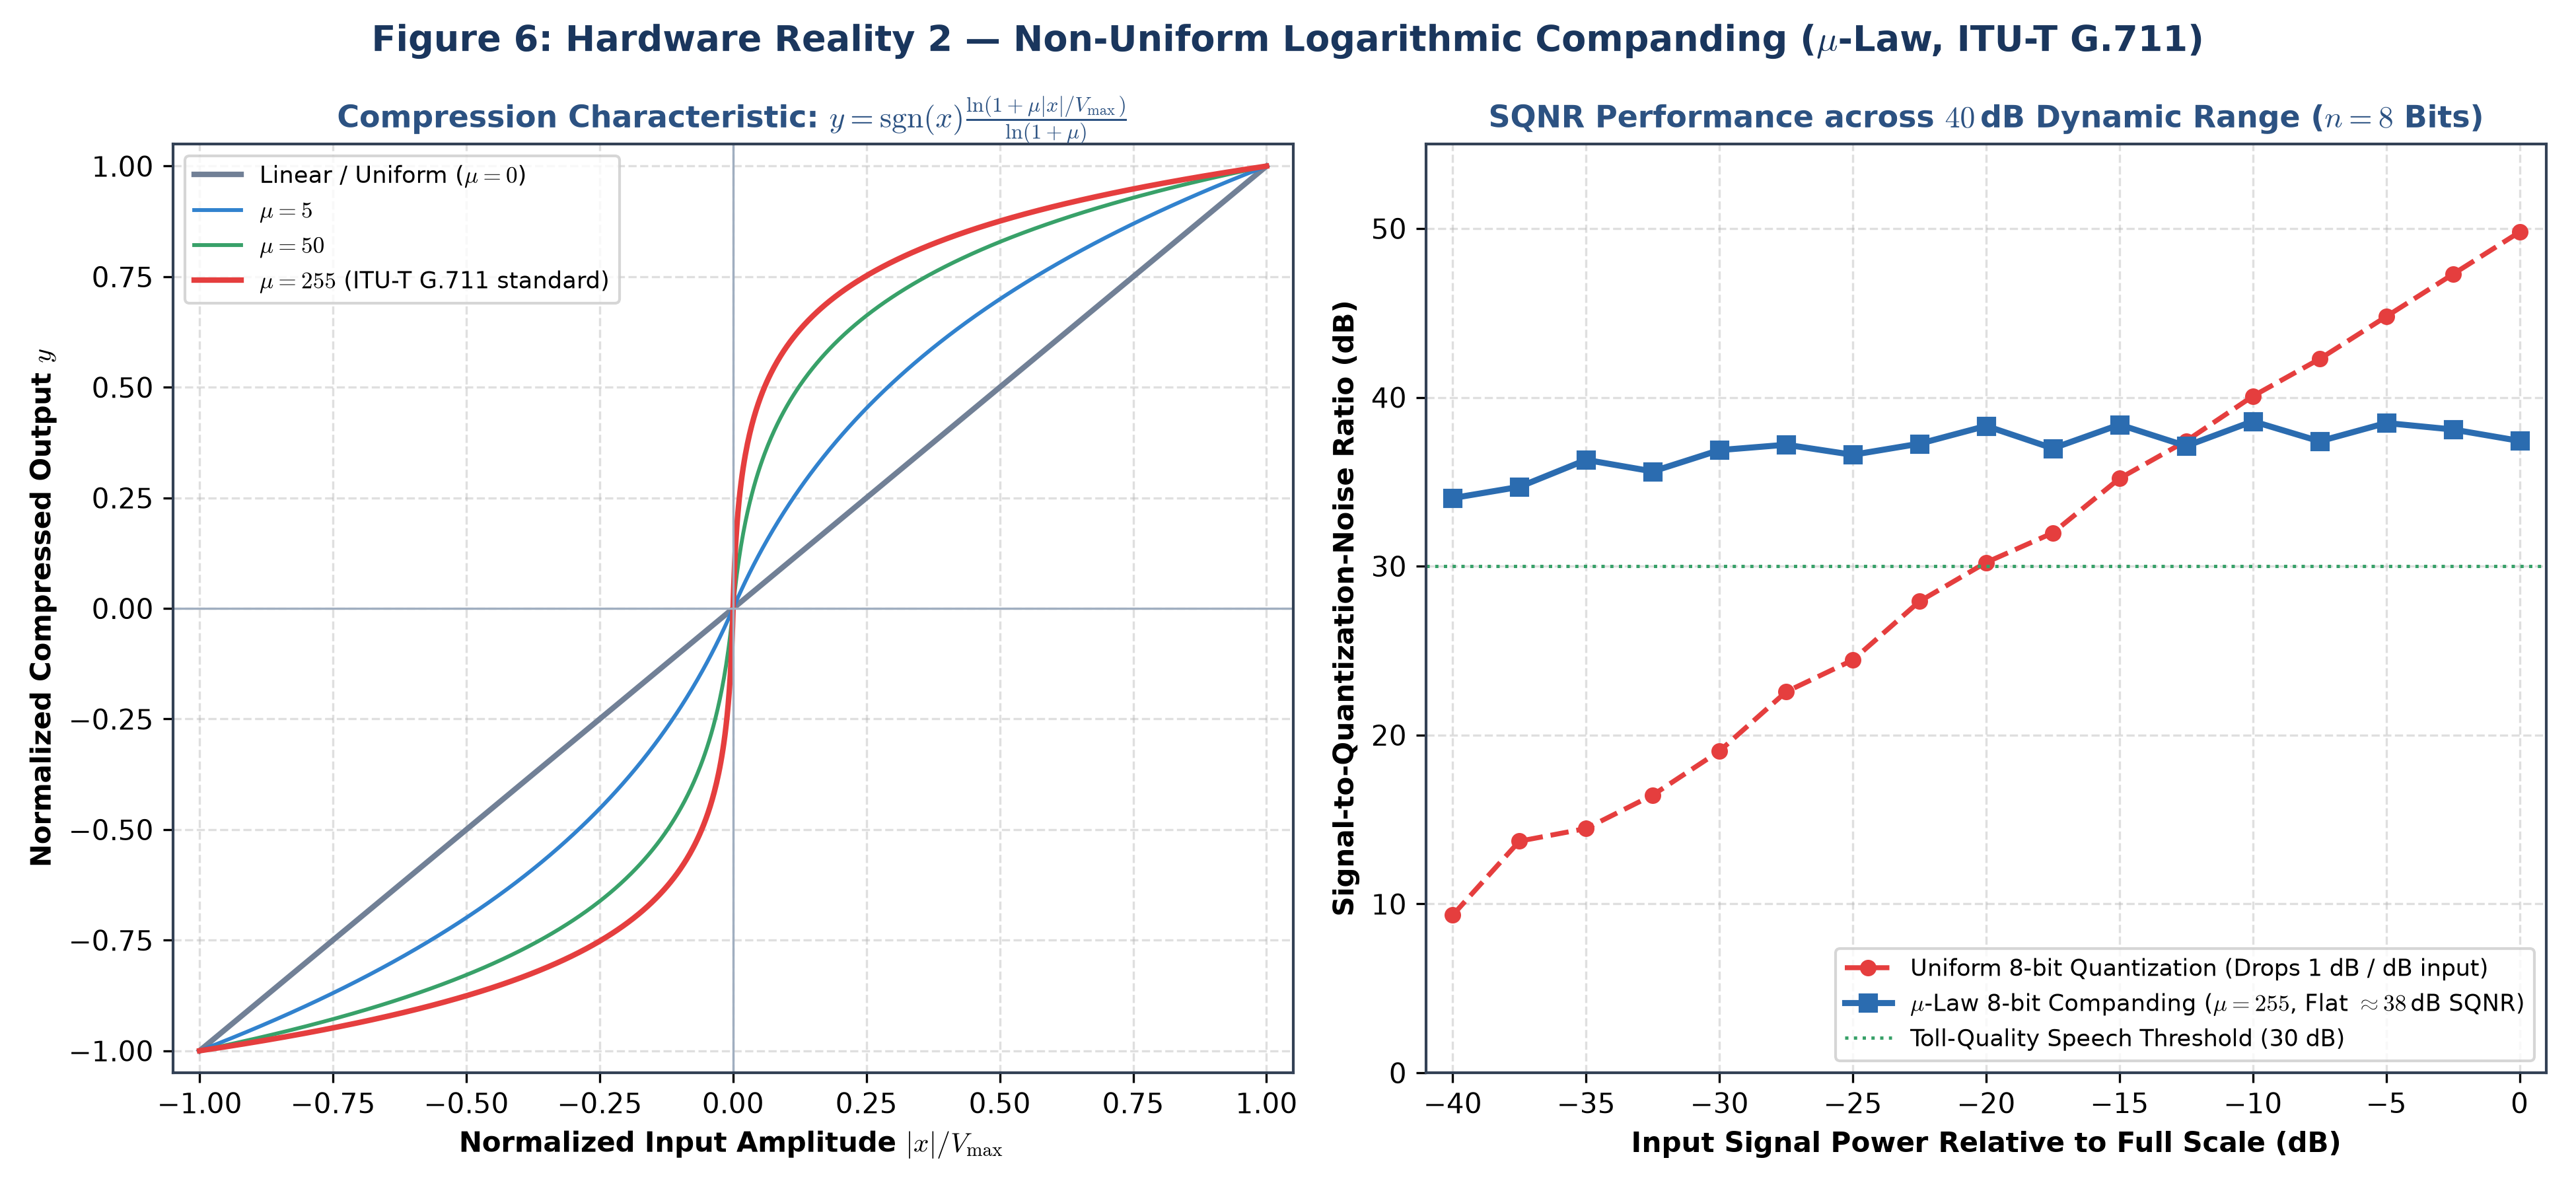
\includegraphics[width=0.88\linewidth]{plots/exp4_companding_mu_law.png}
\caption{Hardware Reality 2: Non-Uniform $\mu$-Law Companding ($\mu = 255$, ITU-T G.711) maintaining constant $\sim 38\,\mathrm{dB}$ SQNR across a $40\,\mathrm{dB}$ dynamic range for speech telephony.}
\end{figure}

\begin{center}
\begin{tabular}{|l|p{5.5cm}|p{6cm}|}
\hline
\textbf{Design Aspect} & \textbf{Pure Mathematical Theory} & \textbf{Practical Engineering Mitigation} \\
\hline
\textbf{Dynamic Range} & Assumes $|x(t)| \le V_{\max}$ strictly & Automatic Gain Control (AGC) \& analog limiting \\
\textbf{Speech Distribution} & Assumes uniform signal power & Logarithmic companding ($\mu$-law / A-law) \\
\textbf{Transmission Bandwidth} & Assumes unconstrained channel bandwidth & Bandwidth trade-off ($B_{\min} = n f_s / 2$) \& DPCM / ADPCM \\
\textbf{Zero Idle Chatter} & Mid-Rise and Mid-Tread identical & Mid-Rise chosen for telephony to silence idle line hiss \\
\hline
\end{tabular}
\end{center}

\newpage

\section{Master Viva-Voce and Conceptual Question Bank (15 Questions)}

\begin{enumerate}
    \item \textbf{Q: What is the fundamental difference between sampling and quantization?}  
    \textbf{A:} Sampling discretizes the continuous \textit{time} axis ($t \to n T_s$) and is mathematically lossless/reversible if $f_s \ge 2 f_{\max}$. Quantization discretizes the continuous \textit{amplitude} axis and is an irreversible, lossy process that introduces permanent error.

    \item \textbf{Q: What is a quantization step size ($\Delta$)?}  
    \textbf{A:} Step size $\Delta$ is the voltage interval between adjacent decision boundaries or representation levels: $\Delta = \frac{2 V_{\max}}{L} = \frac{2 V_{\max}}{2^n}$.

    \item \textbf{Q: Explain the difference between Mid-Rise and Mid-Tread quantizers.}  
    \textbf{A:} In Mid-Rise, the origin ($x=0$) lies on a decision threshold, so there is no representation level at $0\,\mathrm{V}$ (outputs are $\pm \Delta/2, \pm 3\Delta/2, \dots$). In Mid-Tread, the origin lies on a representation level ($0\,\mathrm{V}$ output exists).

    \item \textbf{Q: Why is Mid-Rise preferred in voice/speech PCM telephony?}  
    \textbf{A:} In telephony, background ambient silence contains micro-volt thermal noise. A mid-tread quantizer could oscillate between $0$ and $+\Delta$, causing an audible clicking or hiss. Mid-rise avoids an exact zero state and symmetrically bounds idle noise.

    \item \textbf{Q: Where does the formula $\sigma_e^2 = \frac{\Delta^2}{12}$ come from?}  
    \textbf{A:} Under fine quantization, the error $e$ is uniformly distributed over $[-\Delta/2, +\Delta/2]$ with PDF $f_E(e) = \frac{1}{\Delta}$. Integrating $E[e^2] = \int_{-\Delta/2}^{\Delta/2} e^2 \frac{1}{\Delta} de = \left[ \frac{e^3}{3\Delta} \right]_{-\Delta/2}^{\Delta/2} = \frac{\Delta^2}{12}$.

    \item \textbf{Q: State the 6 dB Rule of PCM.}  
    \textbf{A:} Every additional bit allocated per sample ($n \to n+1$) doubles the number of levels ($L \to 2L$), halves the step size ($\Delta \to \Delta/2$), cuts noise power by $75\%$ ($N_q \to N_q/4$), and increases the SQNR by $10 \log_{10}(4) \approx 6.02\,\mathrm{dB}$.

    \item \textbf{Q: What does the constant $1.76\,\mathrm{dB}$ represent in the formula $\mathrm{SQNR} = 6.02 n + 1.76\,\mathrm{dB}$?}  
    \textbf{A:} It represents $10 \log_{10}(1.5) = 10 \log_{10}(3/2) \approx 1.7609\,\mathrm{dB}$, derived from the ratio of full-scale sinusoidal power ($P_s = V_{\max}^2/2$) to normalized noise power constant ($1/3$).

    \item \textbf{Q: What is the transmission bit rate ($R_b$) of a standard PCM voice channel?}  
    \textbf{A:} Standard voice telephony is bandlimited to $4\,\mathrm{kHz}$, sampled at $f_s = 8\,\mathrm{kHz}$, and quantized with $n = 8$ bits ($L = 256$). Thus, $R_b = n \cdot f_s = 8 \times 8000 = \mathbf{64\,\mathrm{kbps}}$ (standard DS0 channel).

    \item \textbf{Q: What is Quantizer Overload Distortion?}  
    \textbf{A:} When an analog input sample exceeds the quantizer dynamic range ($|x| > V_{\max}$), the quantizer saturates at its maximum level $\pm(V_{\max} - \Delta/2)$. The resulting error exceeds $\Delta/2$ and introduces severe clipping distortion.

    \item \textbf{Q: What is Granular Noise?}  
    \textbf{A:} When the input signal stays within the normal dynamic range ($|x| \le V_{\max}$), the quantization error is strictly bounded within $[-\Delta/2, +\Delta/2]$. This small, distributed error is called granular noise.

    \item \textbf{Q: Why is uniform quantization inefficient for human speech signals?}  
    \textbf{A:} Human speech has a high crest factor; speakers spend most time at very low volume. In a uniform quantizer, low-volume sounds span only a few steps, yielding terrible SQNR (e.g., $10\,\mathrm{dB}$), while loud sounds have high SQNR.

    \item \textbf{Q: What is Companding and how does it solve this problem?}  
    \textbf{A:} Companding (COMpressing + exPANDING) is non-uniform quantization. It compresses the signal logarithmically before uniform quantization (giving fine steps to quiet sounds) and expands it at the receiver, keeping SQNR nearly constant across a $40\,\mathrm{dB}$ dynamic range.

    \item \textbf{Q: Name the two worldwide standard companding laws.}  
    \textbf{A:} 1. \textbf{$\mu$-Law} ($\mu = 255$) used in USA, Canada, and Japan. 2. \textbf{A-Law} ($A = 87.6$) used in Europe, India, and ITU-T international networks.

    \item \textbf{Q: How does DPCM (Differential PCM) improve bandwidth efficiency over standard PCM?}  
    \textbf{A:} Successive analog samples exhibit high correlation ($\rho \approx 0.9$). Instead of quantizing the raw sample $x[k]$, DPCM quantizes only the prediction error $d[k] = x[k] - \hat{x}[k]$. Since $d[k]$ has a much smaller variance, DPCM achieves the same SQNR with $2 - 3$ fewer bits per sample.

    \item \textbf{Q: What is the minimum channel bandwidth required to transmit a binary PCM signal?}  
    \textbf{A:} According to the Nyquist criterion, the minimum baseband transmission bandwidth is $B_{\min} = \frac{R_b}{2} = \frac{n f_s}{2}\,\mathrm{Hz}$. If raised-cosine pulse shaping with roll-off factor $\alpha$ is used, $B = \frac{R_b}{2}(1 + \alpha)$.
\end{enumerate}

\end{document}
